\section{Date: 2026-08-25}
\noindent \textbf{Series ID: G17MVSFAUTOS} 

\noindent This series is titled Regular Seasonal Factors: Auto Production and has a frequency of Monthly. The units are Seasonal Factor and the seasonal adjustment is Not Seasonally Adjusted.The observation start date is 1996-01-01 and the observation end date is 2027-09-01.The popularity of this series is 4. \\ 

\noindent \textbf{Series ID: PATENT4NROREISSUE} 

\noindent This series is titled U.S. Granted Patents: Reissue Patents Originating in Romania and has a frequency of Annual. The units are Number and the seasonal adjustment is Not Seasonally Adjusted.The observation start date is 1993-01-01 and the observation end date is 2020-01-01.The popularity of this series is 1. \\ 

\subsection{Raw Regression}
\noindent Regresses the two series against each other directly. A significant result here can come just as easily from both series sharing a long-run trend as from any real relationship.

\input{tex_tables/regression_table_2026-08-25.tex}

\begin{figure}
\centering
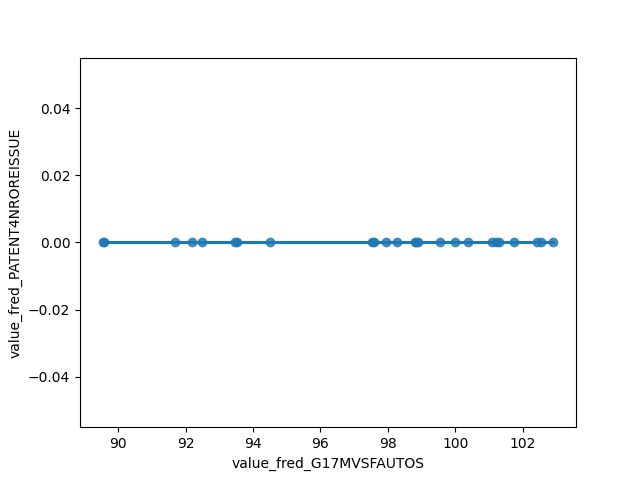
\includegraphics[scale = 0.9]{plots/plot_2026-08-25.png}
\caption{Raw Regression Plot for 2026-08-25}
\end{figure}
\newpage
\subsection{Detrended Regression}
\noindent Regresses the residuals of each series after removing its own linear time trend, so a shared trend can no longer drive the result on its own. A relationship that stays significant here is better evidence of a genuine link between the two series.

\begin{center}
\begin{tabular}{lclc}
\toprule
\textbf{Dep. Variable:}                       & value\_fred\_PATENT4NROREISSUE\_detrended & \textbf{  R-squared:         } &       nan   \\
\textbf{Model:}                               &                    OLS                    & \textbf{  Adj. R-squared:    } &       nan   \\
\textbf{Method:}                              &               Least Squares               & \textbf{  F-statistic:       } &       nan   \\
\textbf{Date:}                                &              Tue, 25 Aug 2026             & \textbf{  Prob (F-statistic):} &      nan    \\
\textbf{Time:}                                &                  12:22:03                 & \textbf{  Log-Likelihood:    } &       inf   \\
\textbf{No. Observations:}                    &                       25                  & \textbf{  AIC:               } &      -inf   \\
\textbf{Df Residuals:}                        &                       23                  & \textbf{  BIC:               } &      -inf   \\
\textbf{Df Model:}                            &                        1                  & \textbf{                     } &             \\
\textbf{Covariance Type:}                     &                 nonrobust                 & \textbf{                     } &             \\
\bottomrule
\end{tabular}
\begin{tabular}{lcccccc}
                                              & \textbf{coef} & \textbf{std err} & \textbf{t} & \textbf{P$> |$t$|$} & \textbf{[0.025} & \textbf{0.975]}  \\
\midrule
\textbf{const}                                &            0  &            0     &       nan  &           nan        &            0    &            0     \\
\textbf{value\_fred\_G17MVSFAUTOS\_detrended} &            0  &            0     &       nan  &           nan        &            0    &            0     \\
\bottomrule
\end{tabular}
\begin{tabular}{lclc}
\textbf{Omnibus:}       &    nan & \textbf{  Durbin-Watson:     } &      nan  \\
\textbf{Prob(Omnibus):} &    nan & \textbf{  Jarque-Bera (JB):  } &      nan  \\
\textbf{Skew:}          &    nan & \textbf{  Prob(JB):          } &      nan  \\
\textbf{Kurtosis:}      &    nan & \textbf{  Cond. No.          } &     3.92  \\
\bottomrule
\end{tabular}
%\caption{OLS Regression Results}
\end{center}

Notes: \newline
 [1] Standard Errors assume that the covariance matrix of the errors is correctly specified.

\begin{figure}
\centering
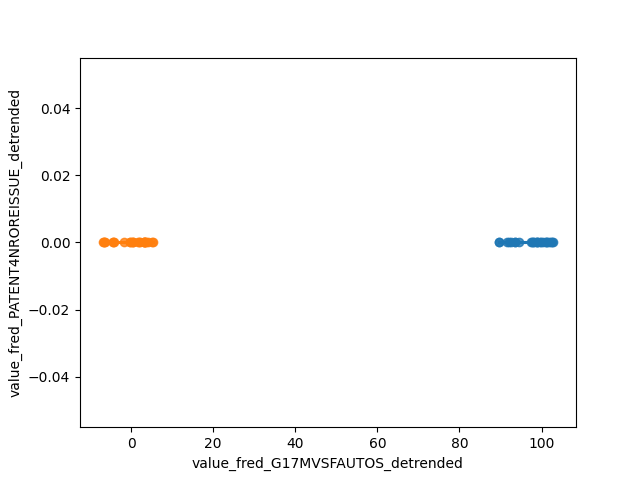
\includegraphics[scale = 0.9]{plots/plot_2026-08-25_detrended.png}
\caption{Detrended Regression Plot for 2026-08-25}
\end{figure}
\newpage
